\section{Résultats}

Comme expliqué précédemment, nous avons exploré plusieurs pistes pour évaluer les performances de notre modèle. L'approche hybride s'est avérée la plus pertinente pour présenter les résultats suivants : elle combine la fiabilité de la vérification par expression régulière pour les questions déterministes à la flexibilité d'un évaluateur LLM (\textit{LLM-as-a-Judge}) pour les questions ouvertes. Notons qu'elle obtient naturellement un score comparable au \textit{LLM-as-a-Judge} dans notre "Benchmark pour Benchmark".

\subsection{Comparaison des Modèles de Langage}

Nous avons évalué la capacité de l'agent à résoudre un benchmark de 27 questions de difficulté variable portant sur la base de code. Le graphique suivant compare le nombre de réponses correctes obtenues selon la configuration du modèle.

\begin{figure}[H]
    \centering
    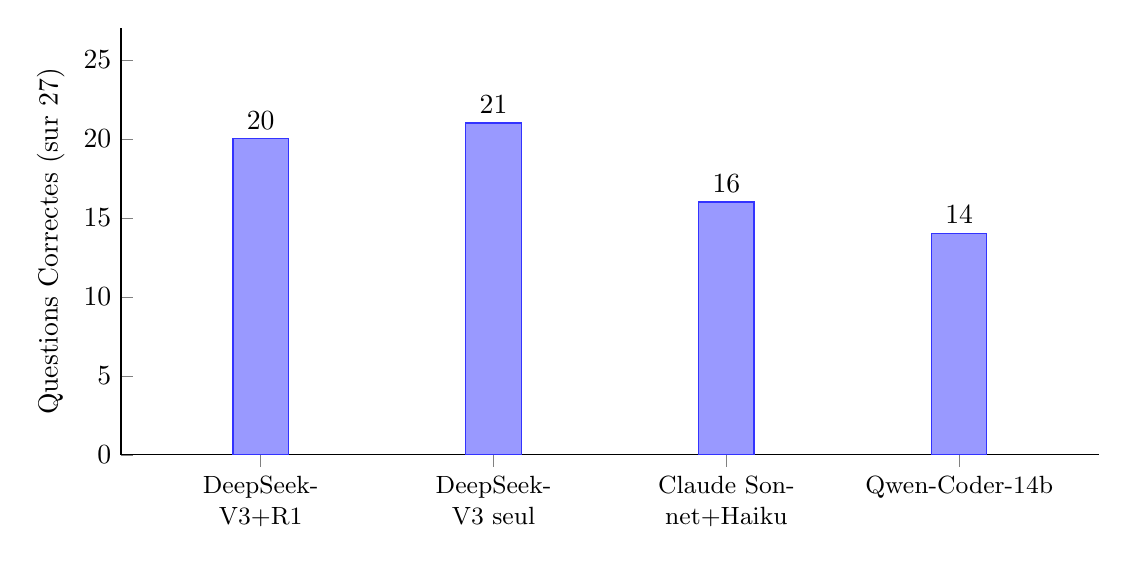
\begin{tikzpicture}
        \begin{axis}[
            ybar,
            bar width=20pt,
            width=14cm,
            height=7cm,
            ylabel={Questions Correctes (sur 27)},
            symbolic x coords={DeepSeek-V3+R1, DeepSeek-V3 seul, Claude Sonnet+Haiku, Qwen-Coder-14b},
            xtick=data,
            ymin=0, ymax=27,
            nodes near coords,
            axis x line*=bottom,
            axis y line*=left,
            enlarge x limits=0.2,
            x tick label style={text width=2.5cm, align=center, font=\small}
        ]
            \addplot[fill=blue!40, draw=blue!80] coordinates {
                (DeepSeek-V3+R1, 20) 
                (DeepSeek-V3 seul, 21) 
                (Claude Sonnet+Haiku, 16) 
                (Qwen-Coder-14b, 14)
            };
        \end{axis}
    \end{tikzpicture}
    \caption{Performance comparative des LLM sur le benchmark de 27 questions.}
    \label{fig:performance_modeles}
\end{figure}

Les meilleurs résultats sont clairement obtenus avec DeepSeek-V3. L'utilisation de DeepSeek-R1 comme \texttt{Solver LLM} offre des performances très similaires, mais allonge significativement le temps d'inférence (+15 \% en moyenne par question). Bien que nos prompts aient été optimisés spécifiquement pour DeepSeek, l'écart de cinq bonnes réponses avec Qwen et Claude confirme la supériorité algorithmique du modèle chinois pour notre cas d'usage.

Ce résultat était prévisible vis-à-vis de \texttt{qwen2.5-coder:14b-instruct}, car DeepSeek-V3 possède 685 milliards de paramètres, lui conférant une capacité de raisonnement et une flexibilité bien supérieures. Toutefois, nous nous attendions à des performances comparables, voire meilleures, de la part de Claude, réputé pour son excellence en analyse et génération de code. Une analyse détaillée de ses échecs révèle que Claude a souvent tendance à halluciner des retours d'outils pour inventer des sources censées étayer ses conclusions. Ce comportement s'explique probablement par notre structuration de contexte, qui diffère drastiquement des conventions standards attendues par les modèles Anthropic. Claude étant un modèle propriétaire, il est très sensible aux écarts de format par rapport à ses données d'entraînement. À l'inverse, les modèles DeepSeek se montrent beaucoup plus agnostiques et résilients face à des formats de prompts atypiques.

Enfin, sur le plan économique, l'exécution complète du benchmark coûte environ 0,15 € avec DeepSeek, contre près de 4 € avec Claude. Étant à la fois plus performant et nettement moins onéreux, DeepSeek-V3 a donc été retenu comme modèle de référence pour construire tous les graphiques suivants.

\subsection{Analyse de l'Utilisation des Outils et de la Latence}

L'agent dispose d'une panoplie d'outils pour explorer le code. La Figure \ref{fig:tool_usage} présente la fréquence d'appel à chaque outil durant la résolution du benchmark, tandis que la Figure \ref{fig:latency_dist} détaille la répartition du temps d'exécution.

\begin{figure}[H]
    \centering
    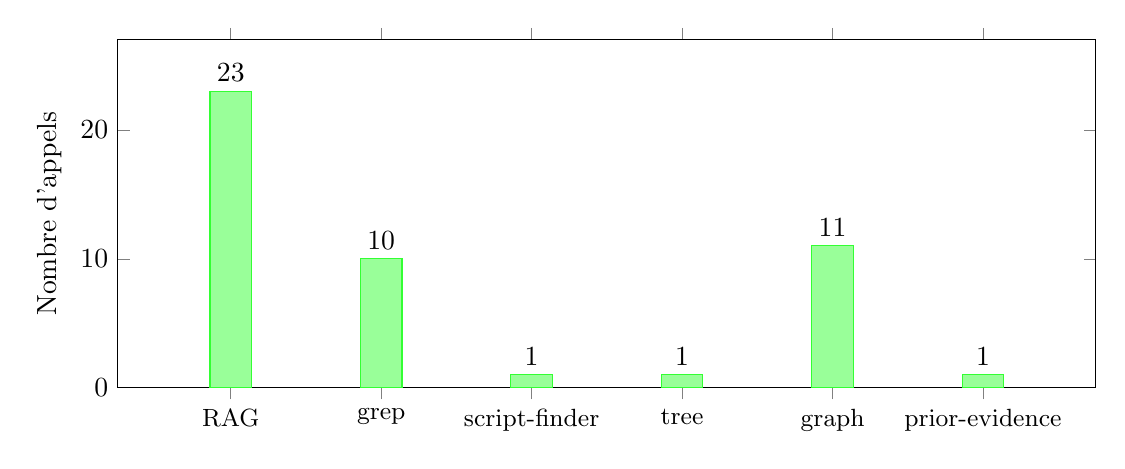
\begin{tikzpicture}
        \begin{axis}[
            ybar,
            bar width=15pt,
            width=14cm,
            height=6cm,
            ylabel={Nombre d'appels},
            ymin=0, ymax=27,
            symbolic x coords={RAG, grep, script-finder, tree, graph, prior-evidence},
            xtick=data,
            nodes near coords,
            enlarge x limits=0.15,
            x tick label style={font=\small}
        ]
            \addplot[fill=green!40, draw=green!80] coordinates {
                (RAG, 23) (grep, 10) (script-finder, 1) (tree, 1) (graph, 11) (prior-evidence, 1)
            };
        \end{axis}
    \end{tikzpicture}
    \caption{Fréquence d'utilisation des outils par l'agent.}
    \label{fig:tool_usage}
\end{figure}

Pour les 7 premières questions du benchmark, fortement axées sur la syntaxe, l'agent utilise quasi exclusivement le \texttt{graph\_tool}. Cet outil étant parfaitement adapté à ce type de recherche, il garantit un taux de réussite systématique de 100 \% sur cette catégorie. Cela explique la concentration des 11 appels sur cet outil, qui n'est ensuite plus sollicité pour le reste de l'évaluation.

Pour les 20 questions restantes, de nature conceptuelles, le RAG devient l'outil de prédilection en raison de sa polyvalence, encore renforcée par nos mécanismes de \textit{boosting} par mots-clés et par sources. Lorsqu'une variable ou un nom de fonction est explicitement mentionné, l'agent effectue souvent une recherche complémentaire via \texttt{grep} pour garantir l'exactitude technique de sa réponse. Enfin, le recours aux autres outils est moins systématique et dépend fortement du cheminement de réflexion adopté par le LLM.

\begin{figure}[H]
    \centering
    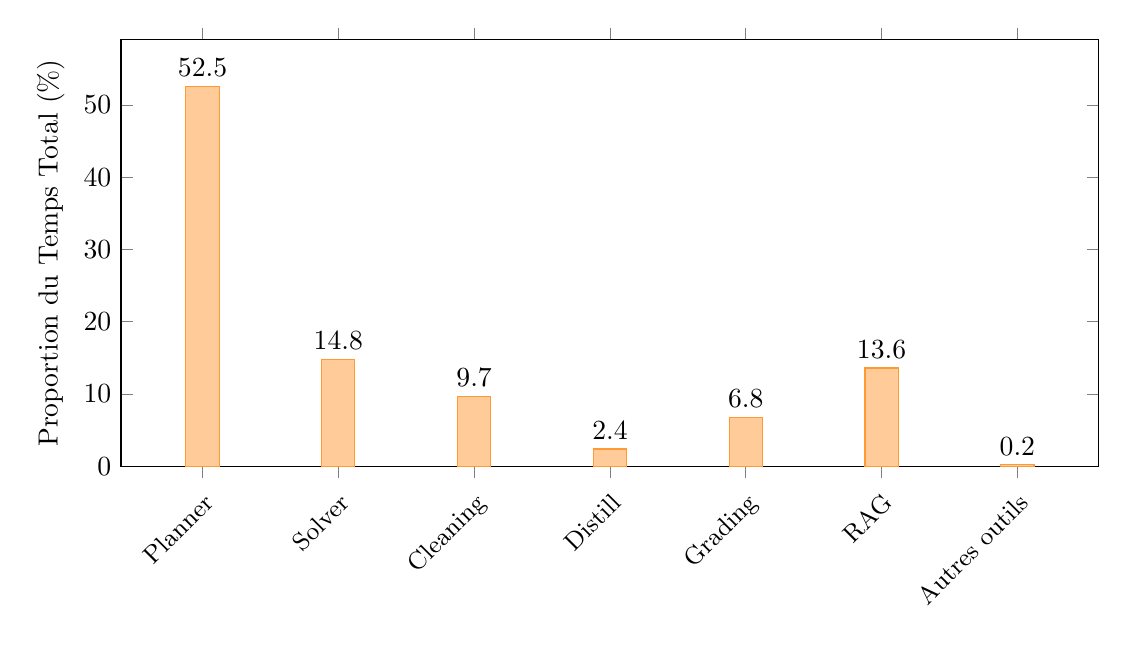
\begin{tikzpicture}
        \begin{axis}[
            ybar,
            bar width=12pt,
            width=14cm,
            height=7cm,
            ylabel={Proportion du Temps Total (\%)},
            ymin=0, ymax=59,
            symbolic x coords={Planner, Solver, Cleaning, Distill, Grading, RAG, Autres outils},
            xtick=data,
            x tick label style={font=\small, rotate=45, anchor=north east},
            nodes near coords,
            enlarge x limits=0.1
        ]
            \addplot[fill=orange!40, draw=orange!80] coordinates {
                (Planner, 52.5) (Solver, 14.8) (Cleaning, 9.7) (Distill, 2.4) (Grading, 6.8) (RAG, 13.6) (Autres outils, 0.2)
            };
        \end{axis}
    \end{tikzpicture}
    \caption{Répartition du temps d'exécution par composant et rôle LLM pour une durée totale de 30m 12s.}
    \label{fig:latency_dist}
\end{figure}

L'analyse de la latence avec DeepSeek-V3 révèle que la majorité du temps d'exécution est monopolisée par le \texttt{Planner LLM}. En tant que centre de commande, ce modèle est chargé de sélectionner les outils à appeler pour explorer la base de code. En décomposant ses 52,5 \% de temps d'exécution, on constate que 27,2 \% sont spécifiquement dédiés à l'évaluation des propositions intermédiaires du \texttt{Solver LLM} (décider si la réponse finale est prête ou si de nouvelles recherches sont requises). Cette étape de vérification est volontairement imposée au système : elle force le LLM à mener une analyse critique avant de proposer une nouvelle action, évitant ainsi des appels d'outils précipités et non pertinents.

Le \texttt{Solver LLM}, chargé de formuler la réponse finale à l'utilisateur, occupe également une portion significative du temps. Cette proportion peut même atteindre 30 \% lorsque l'on utilise DeepSeek-R1, un modèle de raisonnement qui intègre une longue chaîne de pensée (\textit{Chain-of-Thought}) générée directement via l'API.

Enfin, le module RAG a un impact notable sur la latence globale de l'agent (13,6 \%). Comme l'illustre la section suivante, ce délai est presque exclusivement imputable à l'étape de \textit{reranking}, qui sollicite un modèle Transformer lourd pour croiser sémantiquement la requête avec les 25 documents candidats à chaque appel du \texttt{rag\_tool}.

\subsection{Évaluation des Améliorations du RAG}

L'architecture du RAG a évolué pour pallier les limites de la recherche dense simple. Ce graphique présente l'impact de chaque amélioration sur le score de précision final et le temps total passé dans l'outil de RAG pour un benchmark de 20 questions avec DeepSeek-V3 (nous n'avons gardé que les 20 questions conceptuelles sur les 27 questions totales du benchmark car les questions structurelles ne mobilisent pas le RAG).

\begin{table}[H]
    \centering
    \renewcommand{\arraystretch}{1.4} % Aère les lignes du tableau
    \begin{tabular}{l cc cc}
        \toprule
        \textbf{Configuration} & \textbf{Score (sur 20)} & \textbf{$\Delta$ Score} & \textbf{Temps (s)} & \textbf{$\Delta$ Temps (s)} \\
        \midrule
        FAISS & 8 & \textcolor{red}{-6} & 0.47 & \textcolor{green!70!black}{-246.70} \\
        Qdrant-Hybride & 9 & \textcolor{red}{-5} & 2.65 & \textcolor{green!70!black}{-244.52} \\
        % Ligne de référence grisée et en gras
        \rowcolor{gray!15} 
        \textbf{Qdrant+Jina (Réf.)} & \textbf{14} & \textbf{--} & \textbf{247.17} & \textbf{--} \\
        No-Summary & 6 & \textcolor{red}{-8} & 243.05 & \textcolor{green!70!black}{-4.12} \\
        Fusion & 12 & \textcolor{red}{-2} & 519.39 & \textcolor{red}{+272.22} \\
        HyDE & 12 & \textcolor{red}{-2} & 709.18 & \textcolor{red}{+462.01} \\
        \bottomrule
    \end{tabular}
    \caption{Étude d'ablation : évaluation de l'impact des différentes stratégies par rapport à l'architecture de référence.}
    \label{tab:ablation_rag}
\end{table}

Afin d'isoler et de quantifier l'impact de chaque amélioration apportée à notre pipeline de recherche documentaire, nous avons mené une étude d'ablation. En apprentissage automatique, une étude d'ablation consiste à retirer, modifier ou ajouter unitairement des composants d'une architecture complexe afin d'évaluer leur contribution réelle à la performance globale. Le tableau ci-dessus (Table \ref{tab:ablation_rag}) compare six configurations distinctes. La configuration \textit{FAISS} représente notre ligne de base initiale (recherche dense pure). \textit{Qdrant-Hybride} y ajoute la recherche lexicale (BM25) et la fusion RRF. \textit{Qdrant+Jina} introduit l'étape de reranking par Cross-Encoder sur les documents récupérés. L'expérience \textit{No-Summary} reprend cette architecture optimale, mais retire l'utilisation des résumés de code pour l'étape d'embedding, indexant le code brut à la place. Enfin, \textit{Fusion} et \textit{HyDE} testent des stratégies avancées d'augmentation de requêtes par LLM (génération de requêtes multiples pour la première, et génération de document hypothétique pour la seconde).

L'analyse des quatre premiers résultats met en évidence de manière univoque la supériorité de l'architecture combinant Qdrant, le reranking neuronal et l'utilisation de résumés. Le passage de FAISS (8 questions justes sur 20) à Qdrant-Hybride (9/20) montre une légère amélioration grâce au flux sémantique et lexical. Cependant, c'est l'ajout du Cross-Encoder Jina qui crée une véritable rupture technologique, faisant bondir la précision à 14 bonnes réponses sur 20. Ce bond en avant souligne la nécessité d'une analyse profonde du contexte par un Transformer après le premier filtrage vectoriel. Plus important encore, l'expérience \textit{No-Summary} prouve que cette architecture repose fondamentalement sur la qualité de l'indexation initiale : sans les résumés générés pour guider l'embedding (en passant le code brut au modèle d'encodage), le score s'effondre drastiquement à 6/20. L'architecture \textit{Qdrant+Jina} (avec résumés) s'impose donc comme le cœur le plus performant du système, bien qu'il induise naturellement un temps de latence supérieur (environ 247 secondes cumulées pour la résolution des requêtes liées aux 20 questions) lié au coût calculatoire du reranker.

L'évaluation des stratégies d'augmentation de requêtes (\textit{Fusion} et \textit{HyDE}) révèle quant à elle un compromis complexe. Ces deux méthodes atteignent des performances comparables, bien que légèrement inférieures à l'architecture optimale (12 bonnes réponses contre 14). Ce plafonnement s'accompagne surtout d'une explosion significative du temps d'inférence, le processus de génération de LLM supplémentaire propulsant la latence à plus de 519 secondes pour le RAG-Fusion, et au-delà des 709 secondes pour HyDE. Bien que ces méthodes s'avèrent trop coûteuses en temps pour un gain de précision net inexistant, elles présentent un comportement intéressant : les résultats de ces benchmarks ont montré un écart-type plus faible entre les différentes exécutions. En d'autres termes, si RAG-Fusion et HyDE abaissent légèrement le plafond de performance maximale de notre agent, elles semblent le rendre globalement plus prévisible et moins sujet aux variations aléatoires liées à la température des LLM.

\subsection{Analyse détaillée des questions du Benchmark}

Le tableau ci-dessous répertorie les 27 questions du benchmark, catégorisées selon leur nature. Un code couleur indique le niveau de performance de l'agent pour chacune d'elles.

\vspace{0.5cm}

% Définition de couleurs personnalisées (Format HTML ou RGB)
\definecolor{easyColor}{HTML}{cdf7d8} % Vert très clair
\definecolor{intermediateColor}{HTML}{d2ebf7} % Bleu très clair
\definecolor{hardColor}{HTML}{FADBD8}    % Rouge très clair

\begin{longtable}{
    >{\centering\arraybackslash}p{0.08\textwidth} 
    >{\raggedright\arraybackslash}p{0.85\textwidth}
}
\caption{Liste des 27 questions traitées par l'agent RAG.}
\label{tab:questions_benchmark} \\

\toprule
\textbf{N°} & \textbf{Question posée au système} \\
\midrule
\endfirsthead

\multicolumn{2}{c}%
{{\bfseries \tablename\ \thetable{} -- Suite de la page précédente}} \\
\toprule
\textbf{N°} & \textbf{Question posée au système} \\
\midrule
\endhead

\midrule
\multicolumn{2}{r}{{Suite sur la page suivante...}} \\
\endfoot

\bottomrule
\endlastfoot

% --- SOUS-SECTION : SYNTAXIQUE ---
\rowcolor{gray!15}
\multicolumn{2}{c}{\textbf{Questions plutôt Syntaxiques (Recherche de métadonnées et de chemins)}} \\
\midrule
\rowcolor{easyColor} 1  & Combien de scripts lisent /Clean/Items.ion ? \\
\rowcolor{easyColor} 2  & Quels scripts lisent /Clean/Items.ion ? \\
\rowcolor{easyColor} 3  & Combien de scripts lisent /Clean/Forecast/Periodic/FcItems.ion? \\
\rowcolor{easyColor} 4  & Quels scripts lisent /Clean/Forecast/Periodic/FcItems.ion? \\
\rowcolor{easyColor} 5  & Quels scripts écrivent /Clean/Forecast/Periodic/FcItems.ion? \\
\rowcolor{easyColor} 6  & Combien de scripts font mention de /Clean/Forecast/Periodic/FcItems.ion ? \\
\rowcolor{easyColor} 7  & Quels scripts font mention de /Clean/Forecast/Periodic/FcItems.ion ? \\
\midrule

% --- SOUS-SECTION : CONCEPTUELLE ---
\rowcolor{gray!15}
\multicolumn{2}{c}{\textbf{Questions plutôt Conceptuelles (Compréhension de la logique métier)}} \\
\midrule
\rowcolor{easyColor} 8  & Quels sont les modules utilisés ? \\
\rowcolor{intermediateColor} 9  & Où sont calculés les meilleurs vendeurs ? \\
\rowcolor{intermediateColor} 10 & Que fait-on dans ce compte ? \\
\rowcolor{intermediateColor} 11 & Le client veut ajouter une nouvelle localisation pour le dispatch. Où paramétrer le champ ReDispatchCycle propre à cette localisation ? \\
\rowcolor{easyColor} 12 & Existe-t-il une fonction pour calculer l'évolution du stock dans le temps en tenant compte des arrivages et de la demande ? \\
\rowcolor{intermediateColor} 13 & Je vais recevoir une nouvelle colonne FuturSellPrice dans ma table catalogue. Dans quel script effectuer des checks de cohérence sur les valeurs observées ? \\
\rowcolor{easyColor} 14 & Combien de profils de saisonnalité sont appris pour créer le moteur de prévision ? \\
\rowcolor{intermediateColor} 15 & Existe-t-il un endroit où retrouver des informations condensées pour analyser les différents fournisseurs ? \\
\rowcolor{intermediateColor} 16 & Où paramétrer des changements globaux sur les prix de vente afin d'observer leur impact sur la prévision des ventes ? \\
\rowcolor{intermediateColor} 17 & Quelle fenêtre temporelle est prise en compte pour l'apprentissage de la prévision des ventes ? \\
\rowcolor{intermediateColor} 18 & Le produit CT-110-DC est-il traité de façon spécifique dans les scripts ? \\
\rowcolor{hardColor} 19 & Comment sont définies les cibles de fill rate à respecter selon les produits du catalogue ? \\
\rowcolor{intermediateColor} 20 & Comment et où est définie la croissance annuelle pour chaque produit ? \\
\rowcolor{intermediateColor} 21 & Comment définit-on le fait qu'une ref soit une top ref ? \\
\rowcolor{hardColor} 22 & Est-ce que je peux prendre en compte des ventes retour (quantités négatives) dans mes calculs de KPIs ? \\
\rowcolor{hardColor}23 & Est-ce qu'on pondère l'apprentissage des ventes selon leurs dates pour déterminer une prévision future des ventes ? \\
\rowcolor{easyColor} 24 & Comment modélise-t-on le coût de posséder une unité d'un produit en stock ? \\
\rowcolor{intermediateColor} 25 & Est-ce que le client a l'autonomie de paramétrer lui-même la cible de taux de satisfaction de la demande (fill rate) ? \\
\rowcolor{easyColor} 26 & Le client aimerait suivre l'évolution des ruptures de stock : est-ce qu'un dashboard existe déjà qui pourrait être utile ? \\
\rowcolor{easyColor} 27 & Quel type de demande moyenne affiche-t-on au client sur le compte? \\

\end{longtable}

\begin{center}
    \textbf{Légende du Benchmark :} \\ \vspace{0.2cm}
    \fcolorbox{black}{easyColor}{\rule{0pt}{6pt}\rule{6pt}{0pt}} \footnotesize Questions réussies plus de 95\% du temps \quad
    \fcolorbox{black}{intermediateColor}{\rule{0pt}{6pt}\rule{6pt}{0pt}} \footnotesize Questions parfois réussies et parfois non \quad
    \fcolorbox{black}{hardColor}{\rule{0pt}{6pt}\rule{6pt}{0pt}} \footnotesize Questions toujours échouées
\end{center}

On constate que les performances de notre agent sont soumises à une part d'aléa : le score moyen se situe autour de 19 bonnes réponses, mais pourrait théoriquement atteindre 24 sur des exécutions extrêmement favorables. Cette variance s'explique par l'utilisation de températures non nulles lors des requêtes aux modèles de langage. Celle-ci est fixée à 0.05 pour le \texttt{Planner LLM}, qui doit suivre une logique de décision implacable, mais s'élève à 0.3 pour le \texttt{Solver LLM} et le \texttt{Distillation LLM}. Cette marge permet de stimuler la créativité textuelle et d'éviter que les modèles ne restent trop prisonniers des formulations exactes de leur corpus d'entraînement.

Pour comprendre concrètement comment notre système fonctionne, voici un résumé de l'exécution de notre agent sur trois questions aux cheminements de résolution distincts :

\begin{itemize}
    \item \textbf{Question 4 : Quels scripts lisent /Clean/Forecast/Periodic/FcItems.ion ?}\\
    Pour cette question technique, le planificateur (\textit{Planner}) identifie une problématique de dépendance structurelle. Au lieu d'utiliser la recherche sémantique ou textuelle qui pourrait générer du bruit, il opte stratégiquement pour le \texttt{graph\_tool}. L'exécution se déroule en deux temps : un premier appel (\texttt{action: "search"}) localise précisément le nœud correspondant au fichier de données dans le graphe. L'agent enchaîne ensuite avec une requête de voisinage (\texttt{action: "neighbors"}) en filtrant les relations entrantes de type lecture (\texttt{direction: "incoming"}, \texttt{relation\_type: "reads"}). Le graphe retourne alors les trois scripts exacts figurant dans la référence. Constatant que les preuves structurelles sont irréfutables et complètes, l'agent valide la réponse immédiatement sans exploration supplémentaire, garantissant une précision maximale et un score parfait.
    
    \item \textbf{Question 18 : Le produit CT-110-DC est-il traité de façon spécifique dans les scripts ?}\\
    Pour cette requête conceptuelle liée à la logique métier (traitement d'exception sur un SKU particulier), le planificateur rejette l'idée d'une simple recherche d'identifiant et privilégie l'outil sémantique hybride (\texttt{rag\_tool}). Il orchestre sa requête en combinant l'identifiant exact (\texttt{CT-110-DC}) avec des mots-clés d'intention (\texttt{"product", "specific", "treatment"}). Le RAG remonte 5 fragments de code pertinents. Lors de la phase de génération, le LLM analyse ces \textit{chunks} et identifie une règle d'exclusion \textit{hardcodée} dans le script \texttt{Forecast Autodiff.nvn} (lignes 155-157). L'agent rédige alors une réponse affirmative, justifiée par l'extrait de code exact qui censure une période de ventes spécifiques (juin-août 2020) pour ce produit. Le module de vérification (\textit{Logic Check}) valide la solidité des preuves, et le module de nettoyage condense l'explication technique en une réponse fluide, obtenant là encore un score hybride de 1 au benchmark.

    \item \textbf{Question 23 : Est-ce qu’on pondère l’apprentissage des ventes selon leurs dates pour déterminer une prévision future des ventes ?}\\
    Ce troisième cas illustre une limite du système (échec sanctionné par un score de 0). Face à cette question conceptuelle, le planificateur a correctement choisi l'outil \texttt{rag\_tool} en générant des mots-clés pertinents bilingues (\texttt{"pondération", "weight", "date", "apprentissage"}). Le problème survient lors de la récupération (RAG) : le système remonte un chunk mathématiquement exact mais sémantiquement hors-sujet issu du fichier \texttt{Final Forecast Plan.nvn}. Ce fragment détaille la pondération \textit{journalière} pour répartir une prévision déjà calculée, au lieu de la pondération \textit{historique} de l'apprentissage (qui se trouvait dans \texttt{Forecast Autodiff}). Piégé par la forte correspondance lexicale (présence des mots "pondération", "date" et "forecast"), l'agent principal construit un raisonnement détaillé, factuel et parfaitement sourcé... mais qui répond à la mauvaise question. Cet exemple souligne la vulnérabilité du RAG face au vocabulaire polysémique ("pondération" signifiant ici deux concepts algorithmiques très distincts dans Envision) et à la formulation de la question.
\end{itemize}

\subsection{Pistes d'amélioration}

Grâce aux échanges avec Clément Liu et les \textit{Supply Chain Scientists}, nous avons réussi à faire ressortir quelques pistes d'amélioration.

Tout d'abord, parmi les outils, nous avons observé qu'il pourrait être bénéfique de rajouter dans le \texttt{graph\_tool} une liaison entre les scripts et les colonnes. Cet ajout permettrait à l'outil d'être plus polyvalent et ainsi d'être plus utilisé qu'il ne l'est pour le moment.

Aussi, pour améliorer l'utilisabilité des outils, car leur nombre tend à augmenter, il peut être utile de prévoir des descriptions et des paramètres consultables pour limiter le contexte initial et donc mieux guider le \textit{planner}. Dans le contexte initial, une description rapide de l'outil pourrait être faite, tandis que le \textit{planner} pourrait demander des précisions sur un outil avant de l'utiliser, incluant les paramètres et des exemples d'utilisation.

Enfin, pour renforcer la fiabilité des réponses, il serait intéressant d'ajouter une étape supplémentaire de vérification à la fin. Nous pourrions par exemple exiger des sources et rejeter des réponses qui n'ont pas de preuves explicites.
\\

Nous ne pouvons pas oublier le fait que notre solution est très sensible à une modification des prompts des agents. En outre, notre benchmark a été construit et testé de nombreuses fois sur un seul compte client. En un sens, il se peut que la solution proposée risque de n'être spécifique qu'à cette base de données, ou du moins, d'être moins efficace sur une autre base de données (overfitting). Concernant le benchmarking lui même, le \textit{LLM-as-a-Judge} qui est utilisé pour une bonne partie de la notation du benchmark, peut être soumis à un biais d'évaluation car nous l'avons nous-même construit. 

Conscients que nous étions soumis à de tels risques, nous nous sommes tout de même employés à ne pas tomber dans le piège trop facilement en gardant un esprit critique tout au long du projet.